% FedUA-Net -- IWAIT 2027 camera-ready (SPIE format, 4--6 pages incl. references)
\documentclass[]{spie}

\usepackage{amsmath,amssymb}
\usepackage{graphicx}
\usepackage{booktabs}
\usepackage{xcolor}
\usepackage{tikz}
\usetikzlibrary{positioning,fit,arrows.meta,backgrounds,calc}
\usepackage{url}

\newtheorem{proposition}{Proposition}
\newcommand{\refrow}[1]{\textcolor{gray}{#1}}
\renewcommand{\arraystretch}{1.0}
\setlength{\textfloatsep}{7pt plus 2pt minus 2pt}
\setlength{\floatsep}{5pt plus 2pt minus 2pt}
\setlength{\abovecaptionskip}{3pt}
\setlength{\abovedisplayskip}{4pt plus 1pt minus 1pt}
\setlength{\belowdisplayskip}{4pt plus 1pt minus 1pt}

\title{FedUA-Net: Uncertainty-Aware Federated Learning for Multi-Modal Medical Imaging}

\author{Md Tareque Jamil Josh\supit{a,b}, Fernanda Miyuki Yamada\supit{a}, Gabriel Peixoto de Carvalho\supit{c}, and Hiroki Takahashi\supit{a}
\skiplinehalf
\supit{a}Graduate School of Informatics and Engineering, The University of Electro-Communications, Tokyo, Japan;\\
\supit{b}Department of Computer Science and Engineering, Daffodil International University, Dhaka, Bangladesh;\\
\supit{c}Graduate School of Engineering Science, Osaka University, Osaka, Japan
}

\authorinfo{Corresponding author: Md Tareque Jamil Josh, E-mail: j2695005@gl.cc.uec.ac.jp}

\begin{document}
\maketitle

%==========================================================================
\begin{abstract}
Hospitals cannot pool patient scans, and they often differ in imaging modality and diagnostic task, which standard federated learning (FL) does not address. We present FedUA-Net, an uncertainty-aware FL framework for hospitals with disjoint label spaces. Sites share an EfficientNetV2-S/CBAM backbone but keep BatchNorm layers and classifiers private; the server weights hospitals equally, each site fine-tunes locally, and per-site conformal prediction either reports a diagnosis or refers the scan to a clinician. On brain MRI, breast ultrasound and chest X-ray data (29,145 images, 11 classes, 3 seeds), FedUA-Net reaches 93.30\% mean accuracy, above FedAvg and FedBN (92.3\%) and within seed variation of Ditto (93.93\%). It raises the small ultrasound site from 85.5\% to 88.6\% and keeps a 3.4--4.0 point lead over FedBN with only 200 or 100 ultrasound training images. Equal weighting is decisive: with size-proportional weights, ultrasound accuracy collapses to 54--56\% for FedAvg and FedBN. Temperature scaling lowers calibration error by 39\%. The adaptive sets behind the 99\% coverage of our extended abstract would refer over 90\% of scans. We prove that any prediction set containing the top-1 label refers at least $|\text{coverage}-\text{accuracy}|$ of the scans, which explains why never-empty sets over-cover and suggests setting each site's coverage target near its accuracy; least-ambiguous sets then meet a 90\% target with about one label per scan.

\end{abstract}

\keywords{Federated learning, multi-modal medical imaging, personalization, client weighting, calibration, conformal prediction, clinical triage}

%==========================================================================
\section{INTRODUCTION}
\label{sec:intro}

Privacy regulation keeps patient images inside each hospital, and federated learning (FL) trains a shared model by exchanging parameters instead of images\cite{mcmahan2017communication,rieke2020future,guan2024federated}. Most FL methods, including those for non-IID data\cite{litian2020fedprox,lixiaoxiao2021fedbn} and personalization\cite{litian2021ditto,oh2022fedbabu}, assume that every client solves the same task. Real consortia often do not. A neurology centre reads brain MRI, a breast clinic reads ultrasound and a chest unit reads radiographs: imaging physics, image statistics and disease categories all differ, so the hospitals can share only a visual representation. This raises three problems. First, the model must accommodate disjoint label spaces and modality-specific feature statistics. Second, hospitals differ greatly in size: our ultrasound site has 27$\times$ fewer training images than the X-ray site, so size-proportional aggregation\cite{mcmahan2017communication} gives it under 3\% of the weight. Third, deep networks are mis-calibrated\cite{guo2017calibration}. Conformal prediction\cite{angelopoulos2023gentle} offers a coverage guarantee, but a guarantee met by returning several diagnoses per scan gives clinicians little help.

We present FedUA-Net, a federated uncertainty-aware network for hospitals that differ in modality and label space, and contribute: \textbf{(i)} a framework in which hospitals share an EfficientNetV2-S/CBAM backbone, keep BatchNorm layers\cite{lixiaoxiao2021fedbn} and classifiers\cite{arivazhagan2019federated} private, aggregate with equal weights and fine-tune locally, and in which per-site temperature scaling and conformal prediction turn each prediction into an automatic diagnosis or a referral (Fig.~\ref{fig:framework}); \textbf{(ii)} an evaluation on three modalities and 11 classes against five FL baselines and centralised training, including data scarcity and ablations, which shows that equal weighting protects the small site for every method and that local fine-tuning is the decisive component; and \textbf{(iii)} a proof that any prediction set containing the top-1 label refers at least $|\text{coverage}-\text{accuracy}|$ of the scans (Proposition~\ref{prop:referral}). With it, we show why the conformal sets of our extended abstract were clinically uninformative and derive a site-specific rule for choosing the coverage target.

\textbf{Related work.} FedProx\cite{litian2020fedprox} limits client drift, and FedBN\cite{lixiaoxiao2021fedbn} keeps BatchNorm local under feature shift. FedPer\cite{arivazhagan2019federated} and FedBABU\cite{oh2022fedbabu} share a body and personalise the head, which also makes disjoint label spaces trainable, whereas Ditto\cite{litian2021ditto} keeps a personal model regularised towards the global one. Task- and modality-heterogeneous methods address richer settings with larger models: FedHCA$^2$\cite{lu2024fedhca2} handles dense prediction, FedMLP\cite{sun2024fedmlp} partially labelled chest images, and FM$^2$\cite{chen2026fm2} and OmniFM\cite{liu2026omnifm} use mixtures of experts or spectral prompting. Agnostic FL\cite{mohri2019agnostic} and $q$-FFL\cite{li2020qffl} re-weight clients to protect the worst-off; equal weighting is the simplest instance of this idea. Temperature scaling (TS)\cite{guo2017calibration} is the standard post-hoc calibrator, label smoothing\cite{muller2019label} also alters confidence, and FedCal\cite{peng2024fedcal} aggregates client scalers for a shared label space. Among conformal scores, APS\cite{romano2020aps} and RAPS\cite{angelopoulos2021raps} adapt set size to difficulty, and LAC\cite{sadinle2019least} minimises expected set size. Federated conformal prediction pools calibration scores across clients that share labels\cite{lu2023federated}, which is impossible with disjoint labels.

%==========================================================================
\section{METHOD}
\label{sec:method}

\begin{figure}[t]
\centering
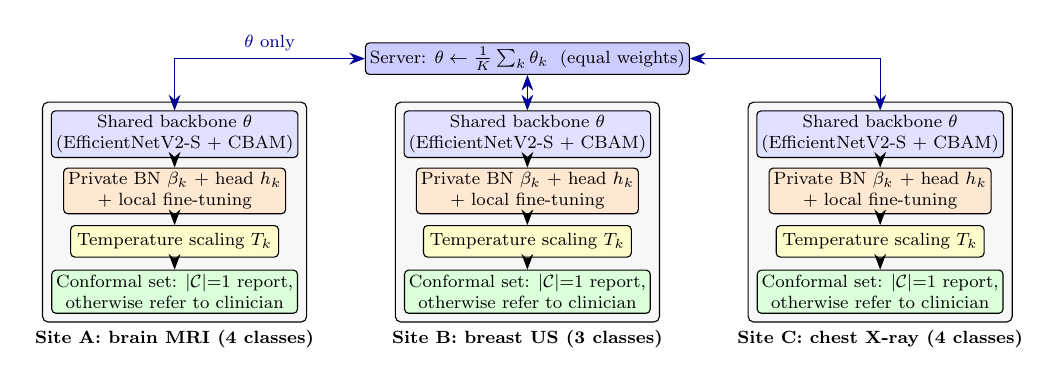
\begin{tikzpicture}[scale=0.8, transform shape,
  font=\footnotesize, >={Stealth[length=2mm]},
  site/.style={draw, rounded corners=2pt, fill=gray!6, inner sep=3pt},
  box/.style={draw, rounded corners=1.5pt, minimum height=5mm, align=center, inner sep=2pt},
  sh/.style={box, fill=blue!12},
  pv/.style={box, fill=orange!18},
  outb/.style={box, fill=green!14}]
  \node[box, fill=blue!20, minimum width=40mm] (srv) at (0,2.1) {Server: $\theta \leftarrow \frac{1}{K}\sum_k \theta_k$ \;(equal weights)};
  \foreach \i/\x/\nm/\ys in {A/-5.6/Site A: brain MRI/4 classes, B/0/Site B: breast US/3 classes, C/5.6/Site C: chest X-ray/4 classes}{
    \node[sh, minimum width=33mm] (F\i) at (\x,0.9) {Shared backbone $\theta$\\ (EfficientNetV2-S + CBAM)};
    \node[pv, minimum width=33mm] (L\i) at (\x,0.0) {Private BN $\beta_k$ + head $h_k$\\ + local fine-tuning};
    \node[box, fill=yellow!20, minimum width=33mm] (C\i) at (\x,-0.8) {Temperature scaling $T_k$};
    \node[outb, minimum width=33mm] (O\i) at (\x,-1.6) {Conformal set: $|\mathcal{C}|{=}1$ report,\\ otherwise refer to clinician};
    \begin{scope}[on background layer]
      \node[site, fit=(F\i)(L\i)(C\i)(O\i), label={[font=\footnotesize\bfseries]below:\nm\ (\ys)}] {};
    \end{scope}
    \draw[->] (F\i) -- (L\i);
    \draw[->] (L\i) -- (C\i);
    \draw[->] (C\i) -- (O\i);
  }
  \draw[<->, blue!60!black] (srv.west) -| node[pos=0.25, above]{$\theta$ only} (FA.north);
  \draw[<->, blue!60!black] (srv.south) -- (FB.north);
  \draw[<->, blue!60!black] (srv.east) -| (FC.north);
\end{tikzpicture}
\caption{FedUA-Net. Only the shared backbone $\theta$ leaves a site; BatchNorm statistics $\beta_k$, the classifier $h_k$, the temperature $T_k$ and the conformal calibration stay private.}
\label{fig:framework}
\end{figure}

\textbf{Model.} Site $k\in\{1,\dots,K\}$ holds $N_k$ labelled images $\mathcal{D}_k$ of modality $m_k$ with label set $\mathcal{Y}_k$, where $\mathcal{Y}_j\cap\mathcal{Y}_k=\emptyset$ for $j\neq k$. It uses $f_k=h_k\circ g_{\theta,\beta_k}$. The backbone $g$ is an ImageNet-initialised EfficientNetV2-S\cite{tan2021efficientnetv2} followed by CBAM channel and spatial attention\cite{woo2018cbam}, global pooling and a 512-d projection with dropout 0.3, and its weights $\theta$ are shared. The BatchNorm parameters and statistics $\beta_k$\cite{lixiaoxiao2021fedbn} and the linear head $h_k$ over $\mathcal{Y}_k$\cite{arivazhagan2019federated} never leave the site.

\textbf{Training.} In round $r$, each site loads the server backbone $\theta^r$, trains $(\theta,\beta_k,h_k)$ for $E_k$ epochs on the class-weighted, label-smoothed ($\epsilon{=}0.1$) cross-entropy over $\mathcal{D}_k$, and returns $\theta^r_k$. The server aggregates
\begin{equation}
\theta^{r+1}=\textstyle\sum_{k=1}^{K}w_k\,\theta_k^{r},\qquad w_k=1/K\ \ \text{(FedUA-Net)}\qquad\text{instead of}\qquad w_k=N_k/\textstyle\sum_j N_j\ \ \text{(FedAvg\cite{mcmahan2017communication})},
\label{eq:agg}
\end{equation}
so a large site cannot dominate the backbone. The last aggregation overwrites each site's backbone with the consensus, so each site then fine-tunes its full model locally for a few epochs and keeps the checkpoint with the best validation accuracy.

\textbf{Calibration and triage.} Each site fits a temperature $T_k$ by minimising the validation negative log-likelihood and predicts $p_k(y\mid x)=\mathrm{softmax}(z/T_k)_y$\cite{guo2017calibration}. Calibration is measured by the expected calibration error (ECE) over 15 equal-width confidence bins. Given $n$ calibration images from site $k$ with scores $s_i=s(x_i,y_i)$, split conformal prediction\cite{angelopoulos2023gentle} returns
\begin{equation}
\mathcal{C}(x)=\{y\in\mathcal{Y}_k:\ s(x,y)\le\hat q\},\qquad \hat q=s_{(\lceil(n+1)(1-\alpha)\rceil)},
\label{eq:cp}
\end{equation}
which guarantees $\Pr[y\in\mathcal{C}(x)]\ge1-\alpha$ for exchangeable data, \emph{separately at each site}. We compare deterministic APS (the score of our extended abstract), randomised APS\cite{romano2020aps}, RAPS\cite{angelopoulos2021raps} ($\lambda{=}0.1$, $k_{\mathrm{reg}}{=}1$) and LAC, \mbox{$s=1-p_k(y\mid x)$}\cite{sadinle2019least}. A singleton set is reported as an automatic diagnosis, and an empty or multi-label set is referred to a clinician.

\begin{proposition}\label{prop:referral}
Let $\mathcal{C}$ be a set predictor whose non-empty sets contain the top-1 label $\hat y(x)$ (true for LAC, APS and RAPS). On any data with top-1 accuracy $a$ and coverage $c$, the referred fraction is at least $|c-a|$. If $\mathcal{C}$ is never empty, then $c\ge a$.
\end{proposition}
\noindent\emph{Proof.} If $\hat y=y$ but $y\notin\mathcal{C}(x)$, the set must be empty; hence $\Pr[\text{empty}]\ge a-c$. If $y\in\mathcal{C}(x)$ but $\hat y\neq y$, the set contains $\hat y$ and $y$; hence $\Pr[|\mathcal{C}|\ge2]\ge c-a$. A never-empty set covers every correct top-1 prediction, so $c\ge a$.\hfill$\square$

\noindent It follows that never-empty predictors (APS, RAPS) must over-cover at any site whose accuracy exceeds $1-\alpha$. For an exact-coverage score such as LAC, referrals are smallest when $1-\alpha$ is close to the site's accuracy.

%==========================================================================
\section{EXPERIMENTAL SETUP}
\label{sec:exp}

\textbf{Data.} Site A: brain tumour MRI\cite{nickparvar2021brain} (glioma, meningioma, no tumour, pituitary; 1,400 training and 400 test images per class, 15\% of training images held out for validation). Site B: BUSI breast ultrasound\cite{aldhabyani2020dataset} (437 benign, 210 malignant, 133 normal; stratified 70/15/15 split). Site C: COVID-19 Radiography\cite{chowdhury2020ai,rahman2021exploring} (3,616 COVID-19, 6,012 lung opacity, 10,192 normal, 1,345 viral pneumonia; 70/15/15). The 29,145 images form 11 disjoint classes. For the scarcity study, site B's 546 training images are subsampled to $N_B\in\{200,100\}$ with validation and test sets unchanged.

\textbf{Baselines and training.} FedAvg\cite{mcmahan2017communication} (BatchNorm shared), FedProx\cite{litian2020fedprox} ($\mu{=}0.01$), FedBN\cite{lixiaoxiao2021fedbn}, FedBABU\cite{oh2022fedbabu}, Ditto\cite{litian2021ditto} ($\lambda{=}1$) and centralised training with an 11-way head. All methods share code, splits, initialisation, the CBAM backbone and private per-site heads, and, unless stated otherwise, equal weights, so FedUA-Net differs from FedBN only in local fine-tuning. As a non-collaborative reference, each site also trains alone for $E_kR$ epochs. Training uses $R{=}12$ rounds, $(E_A,E_B,E_C)=(4,10,2)$ local epochs, AdamW with learning rates $10^{-4}$ (backbone) and $3{\times}10^{-4}$ (head), 2 warm-up rounds, cosine decay and weight decay $10^{-4}$, batch size 32, $224{\times}224$ inputs, random resized crops, flips and colour jitter. Fine-tuning runs for 8/15/5 epochs.

\textbf{Evaluation.} We report per-site and mean accuracy, macro-F1 and ECE as mean$\pm$sd over three seeds, which change both the split and the initialisation, with paired $t$-tests over seeds. Conformal metrics average 500 random 50/50 calibration/test partitions of each site's test set, so calibration and test images are exchangeable. They comprise coverage, set size, referral rate and the accuracy of automatic diagnoses.

%==========================================================================
\section{RESULTS}
\label{sec:results}

\begin{table}[t]
\caption{Test accuracy per site, mean accuracy and macro-F1 over sites (\%, mean$\pm$sd, 3 seeds), and ECE (\%, site mean) before and after temperature scaling. $^\dagger$Temperature fit diverged ($T>5$). Grey: non-collaborative reference.}
\label{tab:main}
\centering\footnotesize\setlength{\tabcolsep}{3.6pt}
\begin{tabular}{lccccccc}
\toprule
Method & A: MRI & B: Ultrasound & C: X-ray & Mean acc. & Macro-F1 & ECE raw & ECE TS \\
\midrule
FedAvg\cite{mcmahan2017communication}   & 96.21$\pm$0.18 & 85.47$\pm$3.08 & 95.39$\pm$0.72 & 92.36$\pm$0.92 & 91.88$\pm$1.23 & 6.97 & 3.98 \\
FedProx\cite{litian2020fedprox}         & 96.12$\pm$0.23 & 84.33$\pm$3.56 & 95.45$\pm$0.67 & 91.97$\pm$1.03 & 91.46$\pm$1.21 & 6.80 & 8.88$^\dagger$ \\
FedBN\cite{lixiaoxiao2021fedbn}         & 96.10$\pm$0.25 & 85.47$\pm$3.42 & 95.44$\pm$0.57 & 92.34$\pm$0.99 & 91.76$\pm$1.02 & 6.50 & 3.79 \\
FedBABU\cite{oh2022fedbabu}             & 96.10$\pm$0.31 & 84.62$\pm$1.48 & 95.24$\pm$0.79 & 91.99$\pm$0.35 & 91.50$\pm$0.34 & 6.40 & 19.13$^\dagger$ \\
Ditto\cite{litian2021ditto}             & 96.15$\pm$0.07 & 90.60$\pm$2.26 & 95.03$\pm$0.99 & 93.93$\pm$0.51 & 93.67$\pm$0.62 & 5.97 & 2.89 \\
Centralised (11-way)                    & 96.38$\pm$0.25 & 88.03$\pm$4.52 & 95.93$\pm$0.66 & 93.45$\pm$1.30 & 93.36$\pm$1.38 & 7.14 & -- \\
\textbf{FedUA-Net (ours)}               & 96.06$\pm$0.29 & 88.60$\pm$3.56 & 95.23$\pm$0.42 & 93.30$\pm$1.13 & 93.05$\pm$1.36 & 5.04 & 3.07 \\
\midrule
\refrow{Local only (reference)}         & \refrow{96.21$\pm$0.10} & \refrow{90.31$\pm$0.99} & \refrow{95.50$\pm$0.43} & \refrow{94.01$\pm$0.32} & \refrow{93.80$\pm$0.48} & \refrow{4.63} & \refrow{2.51} \\
\bottomrule
\end{tabular}
\end{table}

\textbf{Comparison with federated baselines.} In Table~\ref{tab:main}, all methods are within one point of each other at the two large sites and differ almost entirely at the ultrasound site. The methods whose backbone is overwritten by the consensus every round (FedAvg, FedProx, FedBN, FedBABU) reach 84.3--85.5\% there. FedUA-Net's fine-tuning raises site B to 88.6\% and the mean to 93.30\%, improving on FedBN by $+0.96$ points ($p{=}0.047$), FedProx by $+1.33$ ($p{=}0.002$) and FedAvg by $+0.94$ ($p{=}0.16$). Ditto, whose personal models are regularised towards but never overwritten by the global backbone, is the strongest federated method. Its 0.63 point lead is within seed variation ($p{=}0.39$). Central pooling does not help site B either (88.0\%), so the obstacle is limited transfer from MRI and X-ray features to ultrasound, not privacy. Training each site alone gives the highest mean accuracy (94.01\%). We report this reference so that future cross-modality FL methods can be measured against it.

\begin{figure}[t]
\centering
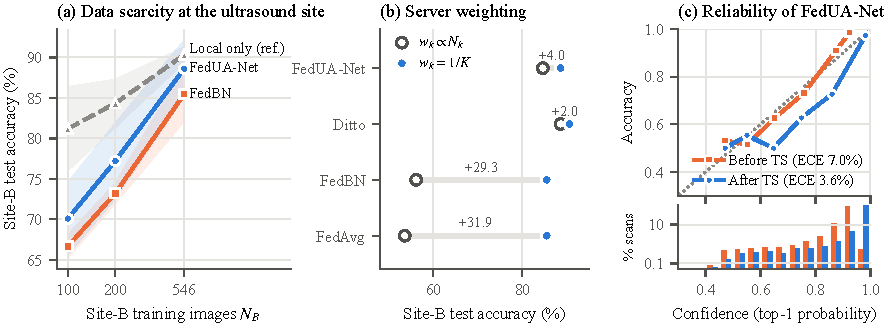
\includegraphics[width=\linewidth]{figures/fig2_results.pdf}
\caption{(a) Site-B accuracy versus its training-set size (mean$\pm$sd, 3 seeds). (b) Site-B accuracy with size-proportional (open) and equal (filled) server weights, with the gain. (c) Reliability diagram of FedUA-Net pooled over sites and seeds (re-run with stored logits), with the share of scans per bin below (log scale).}
\label{fig:results}
\end{figure}

\textbf{What protects the small site.} Figure~\ref{fig:results}(b) isolates the weights of Eq.~\eqref{eq:agg}. With size-proportional weights, site C (74\% of the training images) dominates the backbone, and site B collapses to 53.6\% for FedAvg and 56.1\% for FedBN. Equal weights restore 85.5\% for both, gains of 31.9 and 29.3 points. FedUA-Net (+4.0) and Ditto (+2.0), which adapt the backbone locally, are far less sensitive, so local adaptation and equal weighting are complementary safeguards. Under data scarcity (Fig.~\ref{fig:results}a), FedUA-Net keeps a 4.0 point lead over FedBN at $N_B{=}200$ (77.2\% vs.\ 73.2\%) and 3.4 points at $N_B{=}100$ (70.1\% vs.\ 66.7\%). The gap to isolated training widens (7.1 and 11.1 points), however, because a backbone shaped by MRI and X-ray adapts less well from fewer ultrasound images. A component ablation, run earlier with size-proportional weights, confirms that local fine-tuning is decisive. Removing it reduces site B from 83.5\% to 55.0\% (mean 91.8\% to 82.2\%). CBAM adds 0.6 points at site B, within seed variation.

\textbf{Calibration.} FedUA-Net has the lowest raw ECE of the federated methods (5.04\%), and TS lowers it by 39\% to 3.07\%, comparable to the 42--52\% reductions for FedAvg, FedBN and Ditto. FedUA-Net's temperatures are mostly below one (mean 0.79), so TS \emph{sharpens} the predictions, consistent with label smoothing making raw outputs under-confident\cite{muller2019label}. In Fig.~\ref{fig:results}(c), 80\% of the raw predictions have confidence 0.90--0.95 yet are 98.5\% accurate, and TS moves 90.5\% of the predictions into the top bin. Middle bins, each holding $\le$1.4\% of the scans, deviate more; overall ECE falls from 7.0\% to 3.6\%.

\begin{table}[t]
\caption{Per-site conformal triage for FedUA-Net at $\alpha=0.1$ (target 90\%), averaged over 500 calibration/test partitions and 3 seeds (re-run with stored logits; top-1 accuracy 96.2/86.9/95.6\% at A/B/C). Cov: coverage (\%). Size: mean set size. Ref: referred scans (\%). Auto: accuracy of automatic diagnoses (\%).}
\label{tab:conformal}
\centering\footnotesize\setlength{\tabcolsep}{3pt}
\begin{tabular}{lcccccccccccc}
\toprule
& \multicolumn{4}{c}{A: MRI} & \multicolumn{4}{c}{B: Ultrasound} & \multicolumn{4}{c}{C: X-ray} \\
\cmidrule(lr){2-5}\cmidrule(lr){6-9}\cmidrule(lr){10-13}
Score & Cov & Size & Ref & Auto & Cov & Size & Ref & Auto & Cov & Size & Ref & Auto \\
\midrule
APS, deterministic & 98.7 & 2.26 & 92.3 & 98.9 & 99.5 & 2.31 & 98.7 & 99.5 & 99.7 & 2.27 & 91.6 & 99.0 \\
APS, randomised    & 96.6 & 1.01 & 1.1  & 96.8 & 93.1 & 1.27 & 25.7 & 91.7 & 96.9 & 1.04 & 3.7  & 96.9 \\
RAPS               & 96.4 & 1.01 & 0.5  & 96.5 & 92.0 & 1.22 & 21.8 & 90.7 & 96.2 & 1.02 & 1.7  & 96.2 \\
LAC                & 90.0 & 0.92 & 8.4  & 98.3 & 91.5 & 1.20 & 16.4 & 90.5 & 90.1 & 0.92 & 8.0  & 97.9 \\
\bottomrule
\end{tabular}
\end{table}

\begin{figure}[t]
\centering
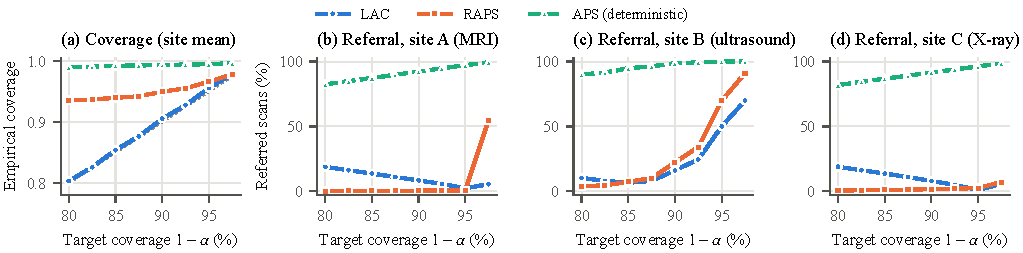
\includegraphics[width=\linewidth]{figures/fig3_conformal.pdf}
\caption{Conformal triage for FedUA-Net versus the target coverage (3 seeds, 300 partitions per point). (a) Coverage averaged over sites; dotted: exact coverage. (b--d) Referred scans per site. LAC referrals are lowest near each site's top-1 accuracy (96.2\%, 86.9\%, 95.6\%), as Proposition~\ref{prop:referral} predicts.}
\label{fig:conformal}
\end{figure}

\textbf{Conformal triage.} Table~\ref{tab:conformal} and Fig.~\ref{fig:conformal} use a re-run of FedUA-Net that stored per-class scores (mean accuracy 92.9\%, site B 86.9\%). Deterministic APS, the score of our extended abstract, reaches 98.7--99.7\% coverage at a 90\% target by returning about two labels per scan and would refer 92--99\% of scans: without randomisation it adds labels until their cumulative probability reaches $\hat q\approx0.98$, and the label-smoothed outputs leave much of that mass on runner-up classes. The 99.1\% of our abstract arose the same way, calibrated on the checkpoint-selection split. Randomised APS and RAPS return about one label but still over-cover at sites A and C (96--97\%): as Proposition~\ref{prop:referral} states, never-empty sets cannot cover less than the top-1 accuracy (96.2\% and 95.6\%). Only LAC meets the target. The excess at site B (91.5\%) is the finite-sample effect of $\lceil(n+1)(1-\alpha)\rceil/n$ with $n\approx58$. LAC refers 8\% of brain and chest scans, all as empty sets that flag images no class explains, and raises the accuracy of the remaining automatic diagnoses from 96.2\% to 98.3\% (A) and from 95.6\% to 97.9\% (C). At site B it refers 16.4\% (bound $|c-a|=4.6\%$). The sweep in Fig.~\ref{fig:conformal} shows a U-shaped LAC referral rate. It refers through empty sets below the site's accuracy and through multi-label sets above it, and it is lowest at a 95\% target for sites A and C (2.4\% and 1.0\%) and at 85\% for site B (6.6\%). A single consortium-wide target is therefore a poor choice: 95\% is nearly free at the MRI and X-ray sites but refers 50\% of ultrasound scans.

%==========================================================================
\section{DISCUSSION AND CONCLUSION}
\label{sec:concl}
Hospitals with different modalities and tasks can train together by sharing only a backbone. Three findings matter for practice. First, aggregation weights decide whether a small specialist site benefits at all: size-proportional averaging erased the ultrasound site for standard methods, and equal weights restored it. Second, local fine-tuning adapts the consensus backbone to a minority modality and makes the model robust to the weighting. Third, coverage alone is a misleading summary of uncertainty. Since sets that contain the predicted label refer at least $|\text{coverage}-\text{accuracy}|$ of the scans, the coverage target should be set per site near its accuracy, and referral rate and automatic-decision accuracy should be reported with coverage.

\textbf{Limitations.} The sites are public datasets standing in for hospitals, so modality and site are confounded, and BUSI and the MRI collection may contain several images per patient, which image-level splits do not control. Three seeds limit statistical power. The component ablation used size-proportional weights, and the calibration and conformal analyses use a re-run of FedUA-Net. Isolated training remains a strong reference at the smallest site, so future work will study consortia in which several hospitals share each modality, and combinations of federated and local models. Code is available at \url{https://github.com/tarequejosh/FedUA-net}.

\bibliographystyle{spiebib}
\bibliography{references}

\end{document}
